\documentclass[9pt,dvipsnames]{beamer}
\usepackage[T1]{fontenc}
\usepackage{libertinus}
\usepackage{amsmath}
\usepackage[most]{tcolorbox}

\usepackage{graphicx}

\usepackage{hyperref}

\usepackage{xcolor}  
\newcommand{\cb}[1]{{\color{CadetBlue}#1}}


\usetheme{Berkeley}
\setbeamertemplate{navigation symbols}{}


\title{CSE574 Introduction to Machine Learning}
\subtitle{Machine Learning: Fundamental Algorithms Part 1}
\author{Jue Guo}
\institute{University at Buffalo}
\date{\today}

\begin{document}
\begin{frame}
    \titlepage
\end{frame}

\begin{frame}
    \frametitle{Outline}
    \tableofcontents
\end{frame}

\begin{frame}{Fundamental Algorithms}
    We will describe \textbf{five algorithms} which are not just the most known but also either very effective on their own or are used as building blocks for the most effective learning algorithms out there.
\end{frame}

\section{Linear Regression}
\begin{frame}{Linear Regression}
	\textbf{Linear regression} is a popular regression learning algorithm that learns a model which is a linear combination of features of the input example.
\end{frame}

\subsection{Problem Statement}
\begin{frame}{Problem Statement}
	We have a collection of labeled examples $\left\{\left(\mathbf{x}_{i}, y_{i}\right)\right\}_{i=1}^{N}$, where $N$ is the size of the collection, $\mathbf{x}_{i}$ is the $D$-dimensional feature vector of example $i=1, \ldots, N, y_{i}$ is a real-valued 
		\footnote{To say that $y_{i}$ is real-valued, we write $y_{i} \in \mathbb{R}$, where $\mathbb{R}$ denotes the set of all real numbers, an infinite set of  numbers from minus infinity to plus infinity.
		} target and every feature $x_{i}^{(j)}, j=1, \ldots, D$, is also a real number.
	
	\begin{itemize}
		\item 	We want to build a model $f_{\mathbf{w}, b}(\mathbf{x})$ as a linear combination of features of example $\mathbf{x}$ :
		
		$$
		f_{\mathbf{w}, b}(\mathbf{x})=\mathbf{w} \mathbf{x}+b
		$$
		
		where $\mathbf{w}$ is a $D$-dimensional vector of parameters and $b$ is a real number. The notation $f_{\mathbf{w}, b}$ means that the model $f$ is parametrized by two values: $\mathbf{w}$ and $b$.
		\item We will use the model to predict the unknown $y$ for a given $\mathbf{x}$ like this: $y \leftarrow f_{\mathbf{w}, b}(\mathbf{x})$. Two models parametrized by two different pairs $(\mathbf{w}, b)$ will likely produce two different predictions 
		when applied to the same example. We want to find the optimal values $\left(\mathbf{w}^{*}, b^{*}\right)$. Obviously,  the optimal values of parameters define the model that makes the most accurate predictions.
	\end{itemize}
\end{frame}

\begin{frame}
	You could have noticed that the form of our linear model is very similar to the form of the SVM model. 
	\begin{itemize}
		\item The only difference is the missing sign operator.
		\item The two models are indeed similar. However, the hyperplane in the SVM plays the role of the decision boundary: it's used to separate two groups of examples from one another. As such, it has to be as far from each group as possible.
	\end{itemize}
	On the other hand, the hyperplane in linear regression is chosen to be as \textcolor{red}{close to} all training examples as possible.
	\begin{figure}
		\centering
		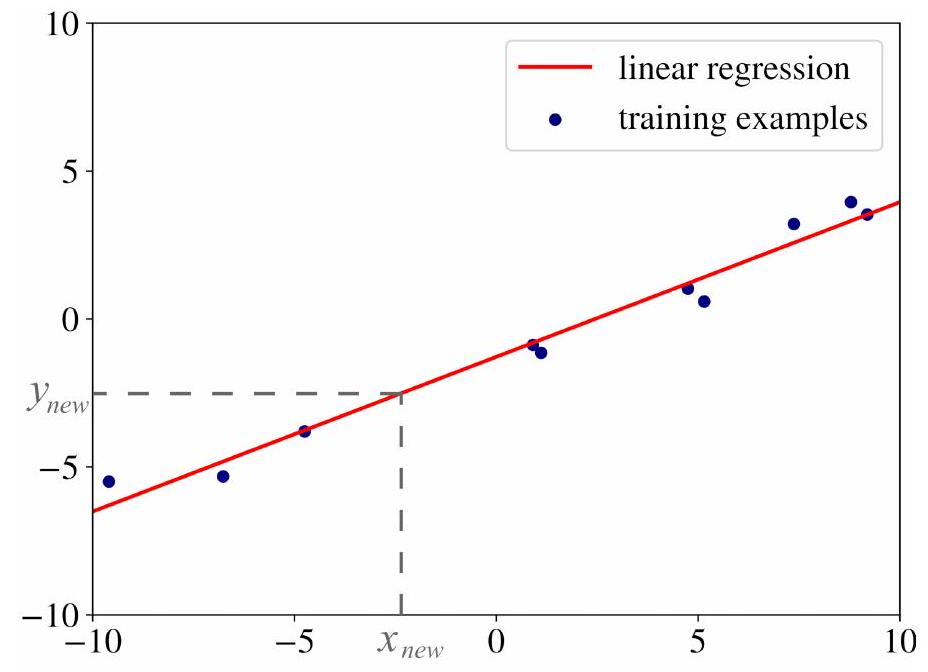
\includegraphics[width=0.4\textwidth]{imgs/algorithm_1.jpg}
		\caption{Linear Regression for one-dimensional examples.}
	\end{figure}
\end{frame}
\begin{frame}
		\begin{figure}
		\centering
		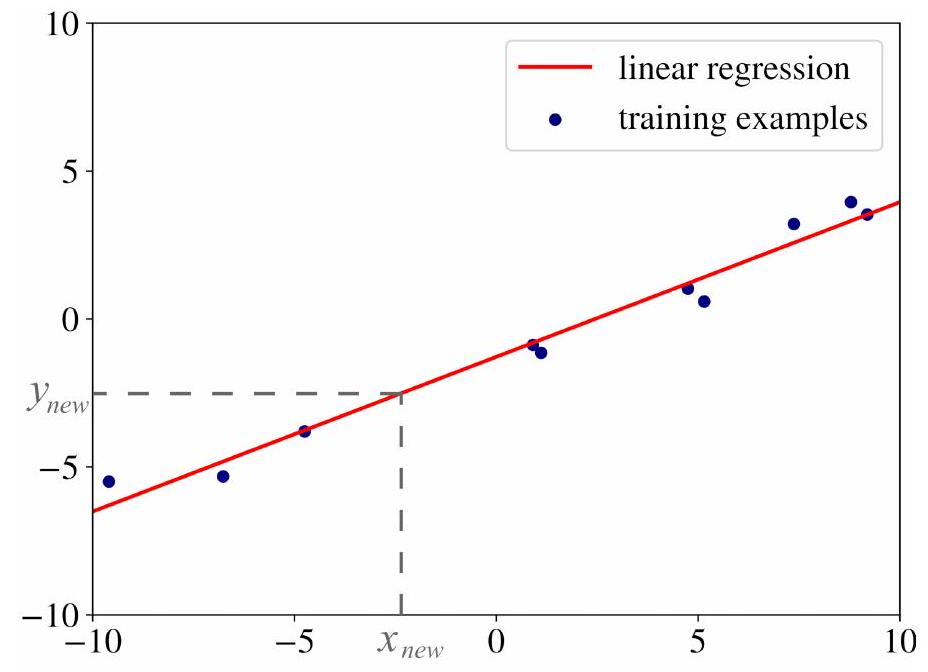
\includegraphics[width=0.4\textwidth]{imgs/algorithm_1.jpg}
		\caption{Linear Regression for one-dimensional examples.}
	\end{figure}
	You can see why this latter requirement is essential by looking at the illustration. It displays the regression line (in red) for one-dimensional examples (blue dots). We can use this line to predict the value of the target $y_{\text {new }}$ for a new unlabeled input example $x_{\text {new }}$.
	\begin{itemize}
		\item If our examples are $D$-dimensional feature vectors (for $D>1$ ), the only difference with the one-dimensional case is that the regression model is not a line but a plane (for two dimensions) or a hyperplane (for $D>2$ ).
	\end{itemize}
	Why it's essential to have the requirement that the regression hyperplane lies as close to the training examples as possible: \textcolor{red}{if the red line was far from the blue dots, the prediction $y_{\text {new }}$ would have fewer chances to be correct.}
\end{frame}
\subsection{Solution}
\begin{frame}{Solution}
	To get this latter requirement satisfied, the optimization procedure which we use to find the optimal values for $\mathbf{w}^{*}$ and $b^{*}$ tries to minimize the following expression:
	
	$$
	\frac{1}{N} \sum_{i=1 \ldots N}\left(f_{\mathbf{w}, b}\left(\mathbf{x}_{i}\right)-y_{i}\right)^{2}
	$$
	In mathematics, the expression we minimize or maximize is called an \textbf{objective function}, or, simply, an \textbf{objective}. 
	\begin{itemize}
		\item The expression $\left(f_{\mathbf{w}, b}\left(\mathbf{x}_{i}\right)-y_{i}\right)^{2}$ in the above objective is called the loss function. It's a measure of penalty for misclassification of example $i$.
		\item This particular choice of the loss function is called \textbf{squared error loss}.
	\end{itemize}
	
   All model-based learning algorithms have a loss function and what we do to find the best model is we try to minimize the objective known as the \textbf{cost function}. 
   \begin{itemize}
   	\item In linear regression, the cost function is given by the average loss, also called the \textbf{empirical risk}. The average loss, or empirical risk, for a model, is the average of all penalties obtained by applying the model to the training data.
   \end{itemize}
\end{frame}

\begin{frame}
	\textbf{Why is the loss in linear regression a quadratic function?}
	\begin{itemize}
		\item Why couldn't we get the absolute value of the difference between the true target $y_{i}$ and the predicted value $f\left(\mathbf{x}_{i}\right)$ and use that as a penalty? We could. Moreover, we also could use a cube instead of a square.
	\end{itemize}
	Now you probably start realizing how many seemingly arbitrary decisions are made when we design a machine learning algorithm: we decided to use the linear combination of features to predict the target. 
	\begin{itemize}
		\item However, we could use a square or some other polynomial to combine the values of features. We could also use some other loss function that makes sense: the absolute difference between $f\left(\mathbf{x}_{i}\right)$ and $y_{i}$ makes sense, the cube of the difference too;	the \textbf{binary loss} (1 when $f\left(\mathbf{x}_{i}\right)$ and $y_{i}$ are different and 0 when they are the same) also makes sense, right?
	\end{itemize}
	
\end{frame}

\begin{frame}
	If we made different decisions about the form of the model, the form of the loss function, and about the choice of the algorithm that minimizes the average loss to find the best values of parameters, we would end up inventing a different machine learning algorithm. Sounds easy, doesn't it? However, do not rush to invent a new learning algorithm. The fact that it's different doesn't mean that it will work better in practice.
	
	People invent new learning algorithms for one of the two main reasons:
	\begin{enumerate}
		\item The new algorithm solves a specific practical problem better than the existing algorithms.
		\item The new algorithm has better theoretical guarantees on the quality of the model it produces.
	\end{enumerate}
	One practical justification of the choice of the linear form for the model is that it's simple. Why use a complex model when you can use a simple one? Another consideration is that linear models rarely overfit.
\end{frame}

\begin{frame}
	\textbf{Overfitting} is the property of a model such that the model predicts very well labels of the examples used during training but frequently makes errors when applied to examples that weren't seen by the learning algorithm during training.
	\begin{figure}
		\centering
		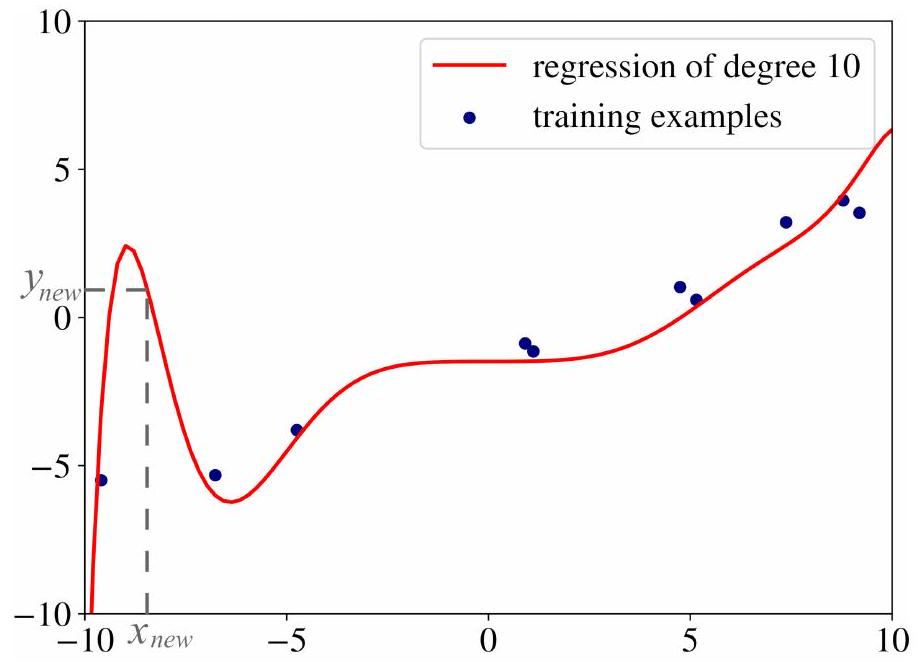
\includegraphics[width=0.4\textwidth]{imgs/algorithm_2.jpg}
		\caption{Overfitting}
	\end{figure}
	The data used to build the red regression line is the same. The difference is that this time, this is the polynomial regression with a polynomial of degree 10 . The regression line predicts almost perfectly the targets almost all training examples, but will likely make significant errors on new data for $x_{n e w}$. We talk more about overfitting and how to avoid it soon.
\end{frame}

\begin{frame}
	Now you know why linear regression can be useful: it doesn't overfit much. But what about the squared loss? Why did we decide that it should be squared? 
	\begin{itemize}
		\item In 1805, the French mathematician Adrien-Marie Legendre, who first published the sum of squares method for gauging the quality of the model stated that squaring the error before summing is convenient.
	\end{itemize}
	 Why did he say that? \textcolor{red}{The absolute value is not convenient, because it doesn't have a continuous derivative, which makes the function not smooth.} Functions that are not smooth create unnecessary difficulties when employing linear algebra to find \textbf{closed form solutions} to optimization problems. 
	 \begin{itemize}
	 	\item Closed form solutions to finding an optimum of a function are simple algebraic expressions and are often preferable to using complex numerical optimization methods, such as \textbf{gradient descent} (used, among others, to train neural networks).
	 \end{itemize}
	Intuitively, squared penalties are also advantageous because \textit{they exaggerate the difference between the true target and the predicted one according to the value of this difference.} We might also use the powers 3 or 4, but their derivatives are more complicated to work with.
\end{frame}

\begin{frame}
	$$
	\frac{1}{N} \sum_{i=1 \ldots N}\left(f_{\mathbf{w}, b}\left(\mathbf{x}_{i}\right)-y_{i}\right)^{2}
	$$
	Finally, \textbf{why do we care about the derivative of the average loss?} 
	\begin{itemize}
		\item 	If we can calculate the gradient of the function in Equation, we can then set this gradient to zero\footnote{To find the minimum or the maximum of a function, we set the gradient to zero because the value of the gradient at extrema of a function is always zero. In 2D, the gradient at an extremum is a horizontal line.} and find the solution to a system of equations that gives us the optimal values $\mathbf{w}^{*}$ and $b^{*}$.
	\end{itemize}
	
\end{frame}
\begin{frame}{A Closed-Form Solution}
	Given the mean squared error (MSE) for a linear model \( f_{\mathbf{w}, b}(\mathbf{x}) = \mathbf{w} \mathbf{x} + b \):
	\[ \text{MSE} = \frac{1}{N} \sum_{i=1}^{N} (\mathbf{w} \mathbf{x}_i + b - y_i)^2 \]
	
	\textbf{Matrix Formulation:} \\
	Rewriting in matrix terms, where \( \mathbf{X} \) is the design matrix and \( \mathbf{y} \) is the vector of target values:
	\[ \text{MSE} = \frac{1}{N} (\mathbf{X}\mathbf{w}^{*} - \mathbf{y})^\top (\mathbf{X}\mathbf{w}^{*} - \mathbf{y}) \]
	
	\textbf{Derivation:} \\
	To minimize the MSE, we differentiate with respect to \( \mathbf{w}^{*} \) and set it to zero:
	\[ \frac{\partial}{\partial \mathbf{w}^{*}} \text{MSE} = 0 \]
	
	This leads to the Normal Equation:
	\[ \mathbf{X}^\top \mathbf{X}\mathbf{w}^{*} = \mathbf{X}^\top \mathbf{y} \]
	
	\textbf{Solving for \( \mathbf{w}^{*} \):} \\
	\[ \mathbf{w}^{*} = (\mathbf{X}^\top \mathbf{X})^{-1} \mathbf{X}^\top \mathbf{y} \]
\end{frame}

\section{Logistic Regression}
\begin{frame}{Logistic Regression}
	The first thing to say is that logistic regression is not a regression, but a classification learning algorithm. 
	\begin{itemize}
		\item The name comes from statistics and is due to the fact that the mathematical formulation of logistic regression is similar to that of linear regression.
		\item I explain logistic regression on the case of binary classification. However, it can naturally be extended to multiclass classification (\textbf{softmax regression}, CSE676 deep learning).
	\end{itemize}
\end{frame}

\subsection{Problem Statement}
\begin{frame}{Problem Statement}
	In \textbf{logistic regression}, we still want to model $y_{i}$ as a linear function of $\mathbf{x}_{i}$, however, with a binary $y_{i}$ this is not straightforward. 
	\begin{itemize}
		\item The linear combination of features such as $\mathbf{w} \mathbf{x}_{i}+b$ is a function that spans from minus infinity to plus infinity, while $y_{i}$ has only two possible values.
	\end{itemize}
	
	At the time where the absence of computers required scientists to perform manual calculations, they were eager to find a linear classification model. 
	\begin{itemize}
		\item They figured out that if we define a negative label as 0 and the positive label as 1 , we would just need to find a simple continuous function whose codomain is $(0,1)$. In such a case, if the value returned by the model for input $\mathbf{x}$ is closer to 0 , then we assign a negative label to $\mathbf{x}$; otherwise, the example is labeled as positive.
	\end{itemize}
\end{frame}

\begin{frame}
One function that has such a property is the \textbf{standard logistic function} (also  known as the \textbf{sigmoid function}):
$$
f(x)=\frac{1}{1+e^{-x}}
$$
where $e$ is the base of the natural logarithm (also called \textit{Euler's number}; $e^{x}$ is also known as the $\exp (x)$ function in programming languages).
\begin{figure}
	\centering
	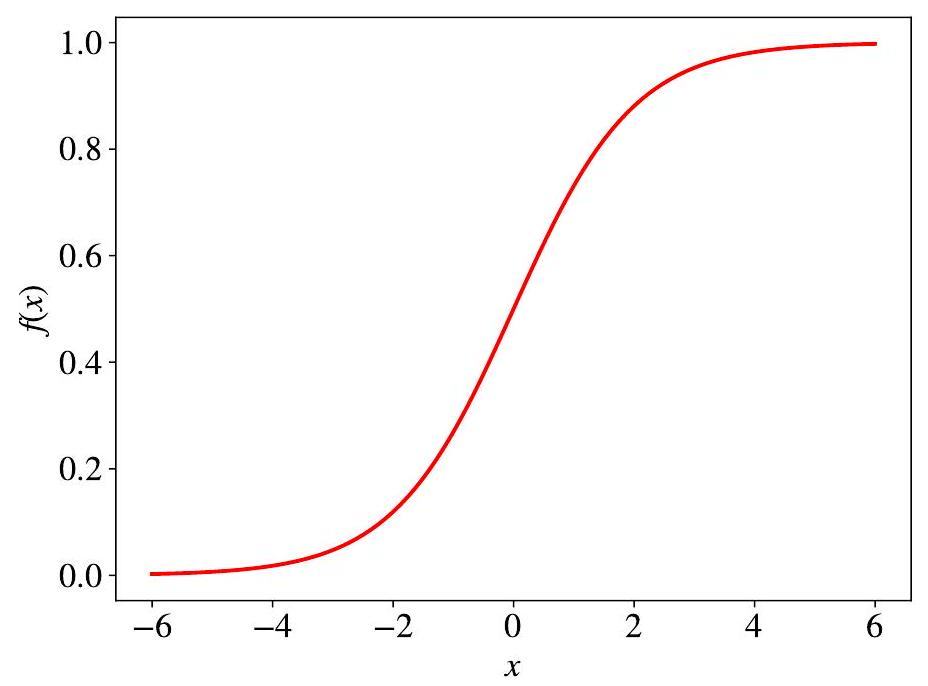
\includegraphics[width=0.5\textwidth]{imgs/algorithm_3.jpg}
	\caption{Standard logistic function}
\end{figure}
\end{frame}

\begin{frame}
	The logistic regression model looks like this:
	
	$$
	f_{\mathbf{w}, b}(\mathbf{x}) \stackrel{\text { def }}{=} \frac{1}{1+e^{-(\mathbf{w} \mathbf{x}+b)}}
	$$
	
	You can see the familiar term $\mathbf{w} \mathbf{x}+b$ from linear regression.
	\begin{figure}
		\centering
		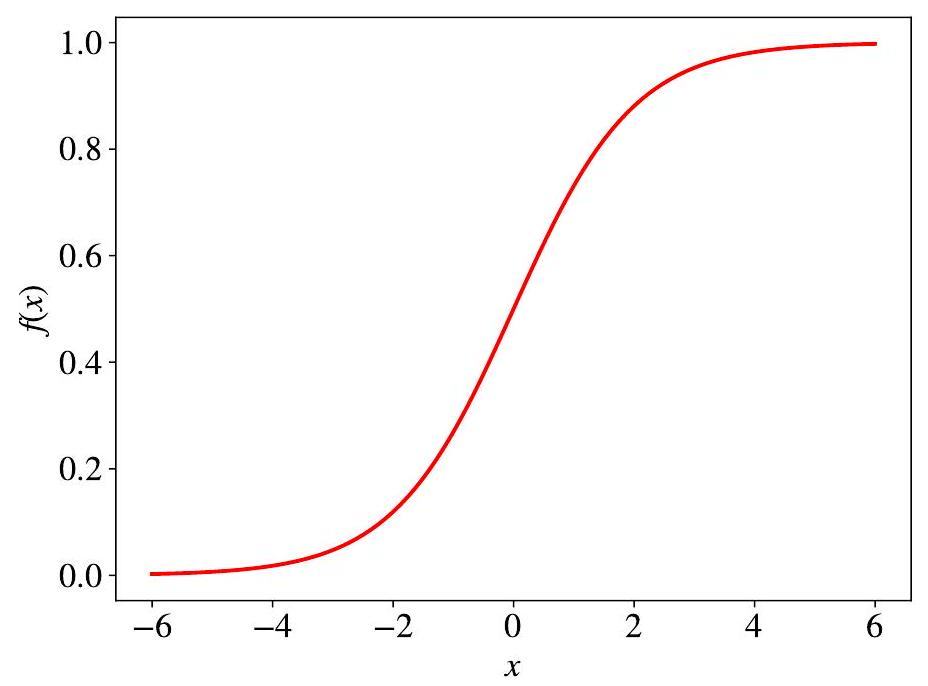
\includegraphics[width=0.3\textwidth]{imgs/algorithm_3.jpg}
		\caption{Standard logistic function}
	\end{figure}
	From the graph, we see how well it fits our classification purpose: 
	\begin{itemize}
		\item if we optimize the values of $\mathbf{w}$ and $b$ appropriately, we could interpret the output of $f(\mathbf{x})$ as the probability of $y_{i}$ being positive. 
	\end{itemize}
	For example, if it's higher than or equal to the threshold 0.5 we would say that the class of $\mathbf{x}$ is positive; otherwise, it's negative. In practice, the choice of the threshold could be different depending on the problem.
\end{frame}

\begin{frame}
	Now, how do we find optimal $\mathbf{w}^{*}$ and $b^{*}$ ? 
	\begin{itemize}
		\item In linear regression, we minimized the empirical risk which was defined as the average squared error loss, also known as the \textbf{mean squared error} or MSE.
	\end{itemize}
\end{frame}
\subsection{Solution}
\begin{frame}{Solution}
	In logistic regression, on the other hand, we maximize the \textbf{likelihood} of our training set according to the model. In statistics, the likelihood function defines how likely the observation (an example) is according to our model.
	\begin{itemize}
		\item For instance, let's have a labeled example $\left(\mathbf{x}_{i}, y_{i}\right)$ in our training data. Assume also that we found (guessed) some specific values $\hat{\mathbf{w}}$ and $\hat{b}$ of our parameters. 
		\item If we now apply our model $f_{\hat{\mathbf{w}}, \hat{b}}$ to $\mathbf{x}_{i}$, we will get some value $0<p<1$ as output. If $y_{i}$ is the positive class, the likelihood of $y_{i}$ being the positive class, according to our model, is given by $p$. Similarly, if $y_{i}$ is the negative class, the likelihood of it being the negative class is given by $1-p$.
	\end{itemize}
\end{frame}

\begin{frame}
	The optimization criterion in logistic regression is called \textbf{maximum likelihood}. Instead of minimizing the average loss, like in linear regression, we now \textcolor{red}{maximize} the likelihood of the training data according to our model:
	
	$$
	L_{\mathbf{w}, b} \stackrel{\text { def }}{=} \prod_{i=1 \ldots N} f_{\mathbf{w}, b}\left(\mathbf{x}_{i}\right)^{y_{i}}\left(1-f_{\mathbf{w}, b}\left(\mathbf{x}_{i}\right)\right)^{\left(1-y_{i}\right)}
	$$
	The expression $f_{\mathbf{w}, b}(\mathbf{x})^{y_{i}}\left(1-f_{\mathbf{w}, b}(\mathbf{x})\right)^{\left(1-y_{i}\right)}$ may look scary but it's just a fancy mathematical way of saying: 
	
	\begin{itemize}
		\item " $f_{\mathbf{w}, b}(\mathbf{x})$ when $y_{i}=1$ and $\left(1-f_{\mathbf{w}, b}(\mathbf{x})\right)$ otherwise".
	\end{itemize}
	 Indeed, if $y_{i}=1$, then 
	$\left(1-f_{\mathbf{w}, b}(\mathbf{x})\right)^{\left(1-y_{i}\right)}$ equals 1 because $\left(1-y_{i}\right)=0$ and we know that anything power 0 equals 1. On the other hand, if $y_{i}=0$, then $f_{\mathbf{w}, b}(\mathbf{x})^{y_{i}}$ equals 1 for the same reason.
\end{frame}

\begin{frame}{}
	\textbf{Example}:
	
	\begin{itemize}
		\item Consider a simple dataset for logistic regression where each input has a corresponding label (0 or 1).
		\item For a given set of parameters:
		\begin{itemize}
			\item If an input is labeled 1 and the model predicts a high probability (close to 1), this contributes positively to the likelihood.
			\item If an input is labeled 0 and the model predicts a low probability (close to 0), this also contributes positively to the likelihood.
		\end{itemize}
		\item By adjusting the parameters to maximize the product of these probabilities across all data points, you're effectively finding the parameter values that make the observed sequence of 0s and 1s most probable according to the model.
	\end{itemize}
	\textbf{Conclusion}
	In essence, "maximize (making the observed data most probable)" means adjusting the logistic regression model's parameters so that the model most accurately represents the actual outcomes observed in the \textbf{training data}. It's a process of aligning the model with the realities of the data it's meant to represent.
\end{frame}

\begin{frame}
	You may have noticed that we used the product operator $\prod$ in the objective function instead of the sum operator $\sum$ which was used in linear regression. It's because the likelihood of observing $N$ labels for $N$ examples is the product of likelihoods of each observation (assuming that all observations are \textit{independent} of one another, which is the case). 
	\begin{itemize}
		\item You can draw a parallel with the multiplication of probabilities of outcomes in a series of independent experiments in the probability theory.
	\end{itemize}
	Because of the $\exp$ function used in the model, in practice, to avoid \textbf{numerical overflow}, it's more convenient to maximize the \textbf{log-likelihood} instead of likelihood. The log-likelihood is defined as follows:
	
	$$
	\log L_{\mathbf{w}, b} \stackrel{\text { def }}{=} \ln \left(L_{\mathbf{w}, b}(\mathbf{x})\right)=\sum_{i=1}^{N}\left[y_{i} \ln f_{\mathbf{w}, b}(\mathbf{x})+\left(1-y_{i}\right) \ln \left(1-f_{\mathbf{w}, b}(\mathbf{x})\right)\right]
	$$
	
	Because ln is a \textbf{strictly increasing function}, maximizing this function is the same as maximizing its argument, and the solution to this new optimization problem is the same as the solution to the original problem. \textit{Contrary to linear regression}, there's no closed form solution to the above optimization problem. A typical numerical optimization procedure used in such cases is \textbf{gradient descent}.
\end{frame}

\begin{frame}
    \begin{center}
        \Huge Questions?
    \end{center}
\end{frame}
\end{document}